%!TEX root = synthese.tex
\newpage
\section{Design Pattern - Singleton}

	\subsection{Objectifs}

	Les objectifs de l'incrément 1 sont les suivants :\\

	\begin{itemize}
	\item Créer un nouvel utilisateur à chaque validation;
	\item Avoir un utilisateur unique par login;
	\item Créer plusieurs terminaux par utilisateur;
	\item Interdir la création d'utilisateur hors de la fenêtre.\\
	\end{itemize}

	Afin de répondre à ces attentes, nous utiliserons le pattern Singleton. Ce pattern s’applique bien à cette situation car la connexion de l’utilisateur est unique. Pour préserver cette unicité, nous allons créer un unique objet représentant la connexion, et stocker la référence à cet objet dans une variable.

	\subsection{Implémentation}

	Le diagramme UML du pattern Singleton se présente sous la forme suivante :

\begin{figure}[!h]
\centering
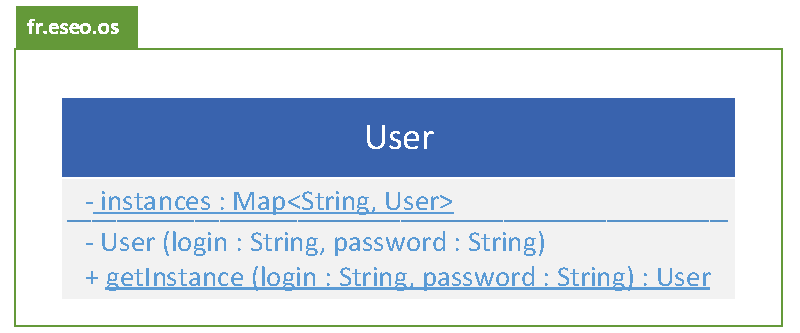
\includegraphics[width=\textwidth]{../uml/uml-singleton}
\end{figure}

On commence par créer un attribut privé et statique qui conserve l’instance de la classe. Cet attribut stockera les utilisateurs déjà créées dans une collection de type \emph{Map}.
\clearpage
\begin{lstlisting}
public class User {
	private String login;
	private String password;
	private static Map<String,User> instances 
									= new HashMap<>();
}
\end{lstlisting}

On crée ensuite une méthode \emph{getInstance()} qui vérifie si l’utilisateur n'existe pas. S'il
n'existe pas, il est ajouté dans la Map \emph{instances} puis retourné. S’il existe, on retourne l’utilisateur existant
que l’on retrouve dans la Map.

\begin{lstlisting}
public synchronized static User 
			getInstance(String login, String password) {
    User user = instances.get(login);
    if (user == null) {
        user = new User(login, password, access);
        instances.put(login, user);
    }
    return user;
}
\end{lstlisting}

Cette méthode est \emph{static} et \emph{public}, ce qui donne un point d'accès universelle à une unique instance.\\

Le mot clé \emph{synchronized} permet de gérer les problématiques d'accès concurrent dans le cas de programmation multitâche. On s'assure ainsi que la ressource ne sera pas partagée à un instant du programme par plusieurs tâches.\\

On définit le constructeur de \emph{User} comme étant privé afin
d’empêcher la création d’objet depuis l’extérieur de la classe.

\begin{lstlisting}
private User(String login, String password){...}
\end{lstlisting}

Enfin, on appelle la méthode \emph{getInstance} dans \emph{TerminalOS} pour créer (ou non) un
nouvel utilisateur associé à un terminal.

\begin{lstlisting}
public TerminalOS(String login, String password){
	super(false);
	this.user = User.getInstance(login, password);
	...
}
\end{lstlisting}

